%%%%%%%%%%%%%%%%%%%%%%%%%%%%%%%%%%%%%%%%%
% a0poster Portrait Poster 
% LaTeX Template
% with University Copenhagen logo
% Version 1.0 (22/06/13)
%
% Based on:
% The a0poster class was created by:
% Gerlinde Kettl and Matthias Weiser (tex@kettl.de)
% 
% This template has been downloaded from:
% http://www.LaTeXTemplates.com
%
%%%%%%%%%%%%%%%%%%%%%%%%%%%%%%%%%%%%%%%%%

%----------------------------------------------------------------------------------------
%	PACKAGES AND OTHER DOCUMENT CONFIGURATIONS
%----------------------------------------------------------------------------------------

\documentclass[a0,portrait]{a0poster}
\usepackage[utf8]{inputenc}
\usepackage{amsmath}	%Para centralizar formulas
\usepackage{multicol} % This is so we can have multiple columns of text side-by-side
\columnsep=45pt % This is the amount of white space between the columns in the poster
\columnseprule=2pt % This is the thickness of the black line between the columns in the poster

\usepackage[svgnames]{xcolor} % Specify colors by their 'svgnames', for a full list of all colors available see here: http://www.latextemplates.com/svgnames-colors

\usepackage{times} % Use the times font
%\usepackage{palatino} % Uncomment to use the Palatino font

\usepackage{graphicx} % Required for including images
\usepackage{tcolorbox} %caixas de texto bacanas
\graphicspath{{figures/}} % Location of the graphics files
\usepackage{booktabs} % Top and bottom rules for table
\usepackage[font=small,labelfont=bf]{caption} % Required for specifying captions to tables and figures
\usepackage{amsfonts, amsmath, amsthm, amssymb} % For math fonts, symbols and environments
\usepackage{wrapfig} % Allows wrapping text around tables and figures

\renewcommand{\refname}{Referências} 
\makeatletter
\newcommand{\eqnum}{\refstepcounter{equation}\textup{\tagform@{\theequation}}}
\makeatother 

\renewcommand{\figurename}{Figura}


\definecolor{ku}{RGB}{144,2,30}	%Título!
\definecolor{ku-yellow}{RGB}{255,249,25}

 \usepackage{eso-pic}
               \newcommand\BackgroundIm{
               \put(66,-71){
               \parbox[b][\paperheight]{\paperwidth}{%
               \vfill
               \centering
               \includegraphics[height=\paperheight,width=\paperwidth,
               keepaspectratio]{background_ufrgs.pdf}%
               \vfill
               }}}

\begin{document}
 \AddToShipoutPicture*{\BackgroundIm}
%----------------------------------------------------------------------------------------
%	POSTER HEADER 
%----------------------------------------------------------------------------------------

% The header is divided into two boxes:
% The first is 75% wide and houses the title, subtitle, names, university/organization and contact information
% The second is 25% wide and houses a logo for your university/organization or a photo of you
% The widths of these boxes can be easily edited to accommodate your content as you see fit



\begin{minipage}[t]{1\linewidth}
\vspace{13.5cm}
\begin{center}
\Huge \color{ku} \textbf{Modelagem e controle de biorreatores anaeróbicos} \color{Black}\\ [1cm]% Title
%\huge\textit{An Exploration of Complexity}\\[1cm] % Subtitle
\Large \textbf{William Cechin Guarienti$^1$, Diego Eckhard$^2$} \\
\vspace{0.5cm}
\color{DarkSlateGray}
\normalsize $^1$\textbf{Estudante de Engenharia de Controle e Automação, UFRGS, Porto Alegre, RS }
williamguarienti@gmail.com\\
\normalsize $^2$\textbf{Professor do Departamento de Matemática Pura e Aplicada, UFRGS, Porto Alegre, RS } diegoeck@ufrgs.br\\[1cm]
\end{center}

\end{minipage}
%
%\begin{minipage}[t]{0.20\linewidth}
%\vspace{14.5cm}
%\flushright
%\color{DarkSlateGray}
%\Large \textbf{Contact Information:}\\
%Øster Farimagsgade 5, 5-1-44\\
%1353 København K\\[1cm]
%Phone: +45 22510702\\ % Phone number
%Email: \texttt{rud.faden@econ.ku.dk}% Email address
%\end{minipage}

\vspace{1cm} % A bit of extra whitespace between the header and poster content

%----------------------------------------------------------------------------------------

\begin{multicols}{2} % This is how many columns your poster will be broken into, a portrait poster is generally split into 2 columns
%setting-the-column-gap-in-a-twocolumn-or-multicol-document???

%----------------------------------------------------------------------------------------
%	ABSTRACT
%----------------------------------------------------------------------------------------

\color{Black} 

%\begin{abstract}
%\end{abstract}

%----------------------------------------------------------------------------------------
%	INTRODUCTION
%----------------------------------------------------------------------------------------

\color{black} % SaddleBrown color for the introduction

\section*{Introdução}
\quad O objetivo deste projeto de pesquisa é estudar um controlador para biorreatores anaeróbicos cujo objetivo é otimizar a síntese de seus produtos.  No caso deste trabalho, o produto de interesse é o gás metano, que é utilizado como combustível em veículos automotores e em plantas industriais.  Utilizando um modelo não linear relativamente simples, foi projetado um controlador PI (proporcional-integral) utilizando a abordagem de espaço de estados. Além disso, são analisados os resultados obtidos com a implementação de tais controladores na planta (biorreator) no software MATLAB. 

\begin{center}\vspace{1cm}
\includegraphics[width=0.4\linewidth]{biorreator.png}
\captionof{figure}{Biorreatores utilizados para a produção dos dados utilizados neste trabalho.}
\label{fig:bioquimica}
\end{center}%\vspace{1cm}


%----------------------------------------------------------------------------------------
%	OBJECTIVES
%----------------------------------------------------------------------------------------
%\color{DarkSlateGray} % DarkSlateGray color for the rest of the content
%\section*{Main Objectives}
%\begin{enumerate}
%\end{enumerate}
%----------------------------------------------------------------------------------------
%	MATERIALS AND METHODS
%----------------------------------------------------------------------------------------
\section*{Modelagem do processo bioquímico}

\quad A digestão anaeróbica de resíduos é um processo no qual microorganismos se desenvolvem a partir do metabolismo de matéria orgânica num ambiente livre de oxigênio, o que resulta na produção de gás metano (CH\textsubscript{4}). Este processo pode ser descrito com aceitável precisão utilizado-se um modelo de baixa complexidade %\cite{walter}
, composto de cinco estados, que permite a estimação da produção de gás metano produzido no biorreator. Admite-se que o único fator limitante para o crescimento dos microorganismos é a disponibilidade de alimento (substrato) e que as demais condições (temperatura, PH, toxidade) são mantidas ideais. 

\quad Os cinco estados do modelo são descritos por:
\begin{gather}
\dot{x_{1}}(t)=[v_{1}(S_{1}(t))-p_7 \cdot D - p_8]\cdot x_1(t)\\
\dot{x_{2}}(t)=[v_{2}(S_{2}(t))-p_7 \cdot D - p_9]\cdot x_2(t)\\
\dot{S_{1}}(t)=D\cdot(S_{1}^{in} - S_{1}(t)) - p_{10} \cdot v_{1}(S_{1}(t))\cdot x_1(t)\\
\dot{S_{2}}(t)=D \cdot (S_{2}^{in} - S_{2}(t)) + p_{11}\cdot v_{1}(S_{1}(t)) \cdot x_1(t) - p_{12} \cdot v_{2}(S_{2}(t)) \cdot x_2(t) \\
\dot{C}(t)= p_{14} \cdot v_{1}(S_{1}(t)) \cdot {x_{1}}(t) + p_{16} \cdot v_{2}(S_{2}(t)) \cdot {x_{2}}(t) - p_{15} \cdot C(t)
\end{gather}
\quad As funções $v_1(t)$ e $v_2(t)$ expressam a velocidade do crescimento bacteriano. Com o intuito de simplificar o problema, tais velocidades foram expressas em conformidadade com a Lei de Monod, que define a taxa de crescimento apenas em função da concentração de substrato:
\begin{equation}
v_i = p_{3i-2}\frac{S_i(t)}{p_{3i-1}+S_1(t)}  \hspace{2cm} i=1,2
\end{equation}
\quad A saída do modelo é a vazão de gás metano, expressa por: $q_m(t)$:\\
\begin{equation}
q_m(t) = p_{13}\cdot v_{2}(S_{2}(t)) \cdot x_2(t) + p_{15} \cdot C(t)
\end{equation}
\quad A seguir, elucidamos o significado das variáveis do modelo:
\begin{itemize}
\item $x_1(t)$: concentração de bactérias acinogênicas [mg/L];
\item $x_2(t)$: concentração de bactérias metanogênicas [mg/L];
\item $S_1(t)$: concentração de substrato orgânico (COD) [mg/L];
\item $S_2(t)$: concentração dos ácidos graxos voláteis (VFA) [mmol/L];
\item $C(t)$: concentração de carbono inorgânico (mmol/L)
\item $S_1^{in}$: concentrações de substrato orgânico dos influentes;
\item $S_2^{in}$: concentrações de ácidos graxos voláteis (VFA) dos influentes;
\item $D$: taxa de diluição dos influentes;
\end{itemize}
\quad Os parâmetros denotados por $p_i$ correspondem a constantes determinados através de um procedimento de identificação com base em dados experimentais, utilizando algoritmos como o \textit{simplex Nelder-Mead} e o \textit{Trust-Region-Reflective}. Define-se, nesse contexto, o vetor linha de parâmetros $P = (p_{1i})$ sendo $i=1,2,...,16$;

%----------------------------------------------------------------------------------------
%	RESULTS 
%----------------------------------------------------------------------------------------

\section*{Controle do processo}
\quad O sistema de controle deve atuar de forma a garantir a manutenção do fluxo adequado de substrato ($S_1^{in}$) para a obtenção da vazão de gás metano desejada ($r(t)$), assumida constante. Para este trabalho, assumiu-se que a taxa de diluição dos influentes é constante e igual a $D = 1 \hspace{1mm} dia^{-1}$; além disso, a concentração de ácidos graxos nos influentes é nula ($S_2^{in} = 0$). A Figura \ref{malha} apresenta o diagrama do sistema de controle associado ao biorreator em questão.  
\begin{minipage}{.5\textwidth}
\begin{center}
\includegraphics[width=0.7\linewidth]{malha.png}
\captionof{figure}{Diagrama do sistema de controle associado ao biorreator} \label{malha}
\end{center}
\end{minipage}

\quad Para os cálculos subsequentes, foi considerado o vetor de coeficientes \textbf{P} da Equação \ref{eq:p}. O procedimento é claramente passível de generalização para qualquer taxa de diluição $D$ e qualquer vetor factível de parâmetros  \textbf{P}; no entanto, tal abordagem levaria a expressões demasiadamente complexas, a partir das quais não se poderia desenvolver a sua adequada compreensão.
\vspace{1mm}
\begin{tcolorbox}	
							
$P = [ 2.74   ;   
      257.17  ;    
      0          ;           
      37.34     ; 
      455.16     ; 
      0           ; 
      0           ;  
      0.0029      ;  
      0.0015      ;  
      32.24     ;  
      28.31     ;  
      100         ;  
      141.99    ; 
      3.93     ;  
      10.71     ;  
      200       ] $  \hspace{4mm}	\eqnum\label{eq:p}
   
\end{tcolorbox}
\vspace{1mm}
\quad A partir do conjunto de parâmetros acima, pode-se efetivamente estudar um controlador para o processo. Arbitrou-se $r = 1 L/dia$ como referência para a variável de processo ($q_m$). Inicialmente, o ponto de equilíbrio do sistema para a geração foi determinado numericamente,
%\begin{equation}
%x_{eq} = [x_1 \hspace{3mm}
% x_2 \hspace{3mm}
% S_1 \hspace{3mm} 
% S_2 \hspace{3mm} 
% C]^T = 
% [3.637 \hspace{3mm}
%1.869 \hspace{3mm}
%0.272 \hspace{3mm}
%0.0183 \hspace{3mm}
%0.0562 \hspace{3mm}]^T
%\end{equation}
e o sistema foi linearizado em dois pontos de operação distintos: em torno da condição inicial ($x_0$) e em torno do ponto de equilíbrio calculado ($x_{eq}$). Na sequência, foram traçados os Diagramas de Bode correspondentes, que são exibidos sobrepostos na Figura \ref{bode}.

\begin{center}
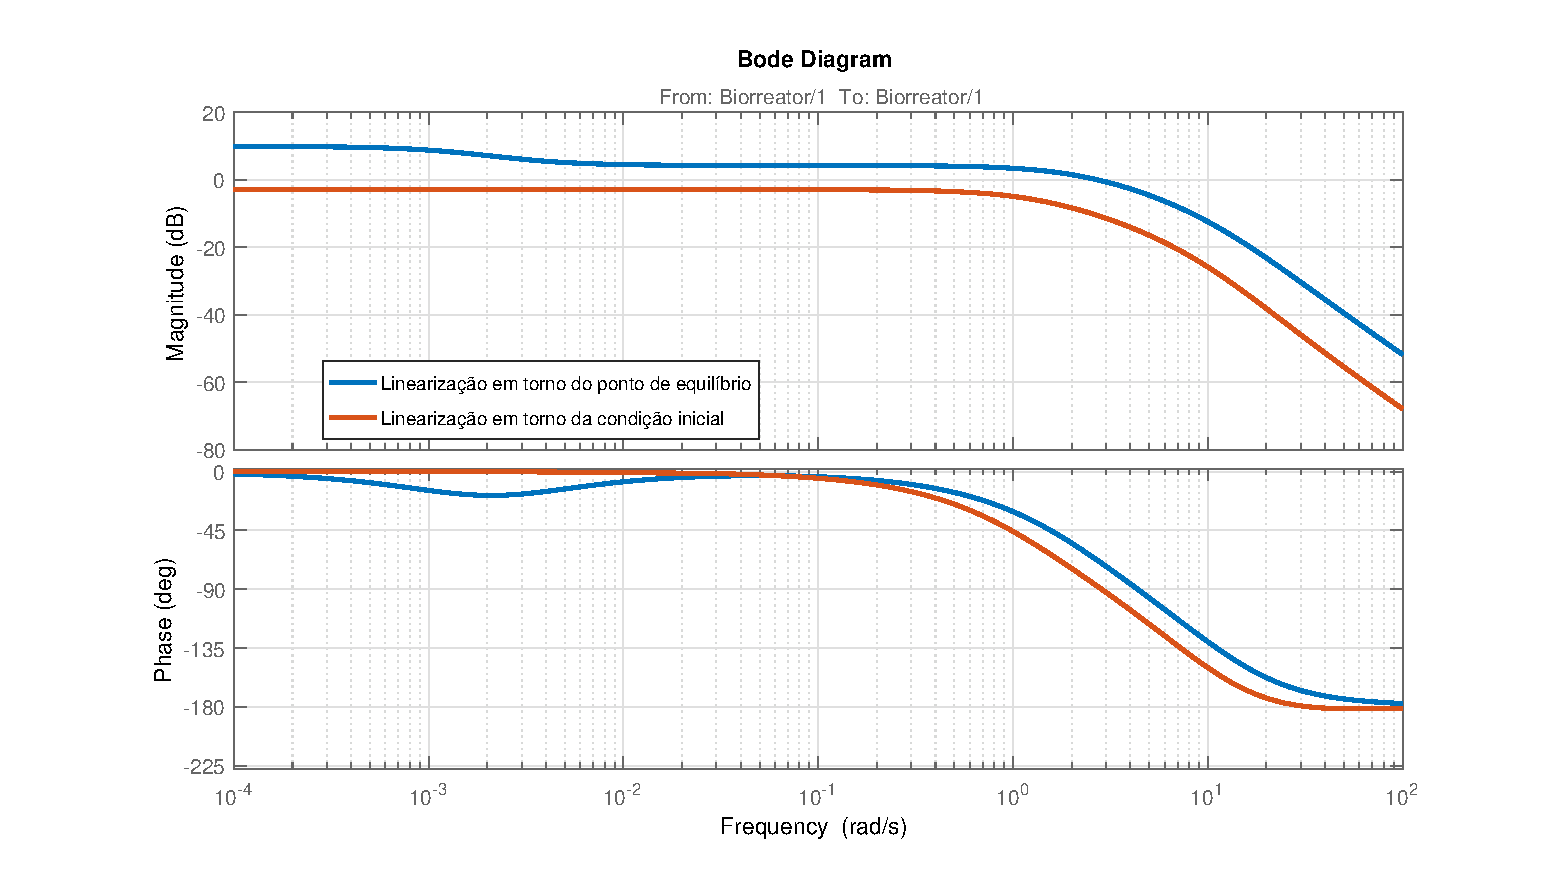
\includegraphics[width=1\linewidth]{bode.eps}
\captionof{figure}{Diagrama de Bode dos sistemas linearizados} \label{bode}
\end{center}
\quad Para o controle do processo, foi implementado um controlador PI na forma padrão (\textit{standard}). Com auxílio dos diagramas traçados acima, foi projetado um que garantisse uma margem de fase mínima de $60^\circ$ e uma margem de ganho mínima de $20dB$ para ambos os modelos. A lei de controle do controlador PI escolhido, que satisfaz as condições enunciadas, é apresentado na Equação \ref{PI}. Verificando o espectro da matriz Jacobiana no ponto de equilíbrio ($x_{eq}$), pode-se corroborar a estabilidade do sistema, visto que a parte real de todos os seus autovalores é negativa (\textit{Lyapunov's indirect method}).
\begin{gather}
S_1^{in} (t) =  0.143 \cdot (r(t)-q_m(t)) + 1 \cdot \int_{0}^{t} r(\tau)-q_m(\tau) d\tau  \label{PI}
\end{gather} 
   
\section*{Resultados}

\quad Conforme é exibido na Figura \ref{sim}, o sistema em malha fechada - com o controlador descrito pela Equação \ref{PI} - obteve tempo de estabilização significativamente menor do que o sistema em malha aberta. Além disso, observa-se que o esforço de controle ($S_1^{in} (t)$) manteve-se em níveis razoáveis. Caso seja necessário, um ajuste fino dos parâmetros pode ser feito para reduzir o sobressinal observado no sistema em malha fechada.

\begin{center}
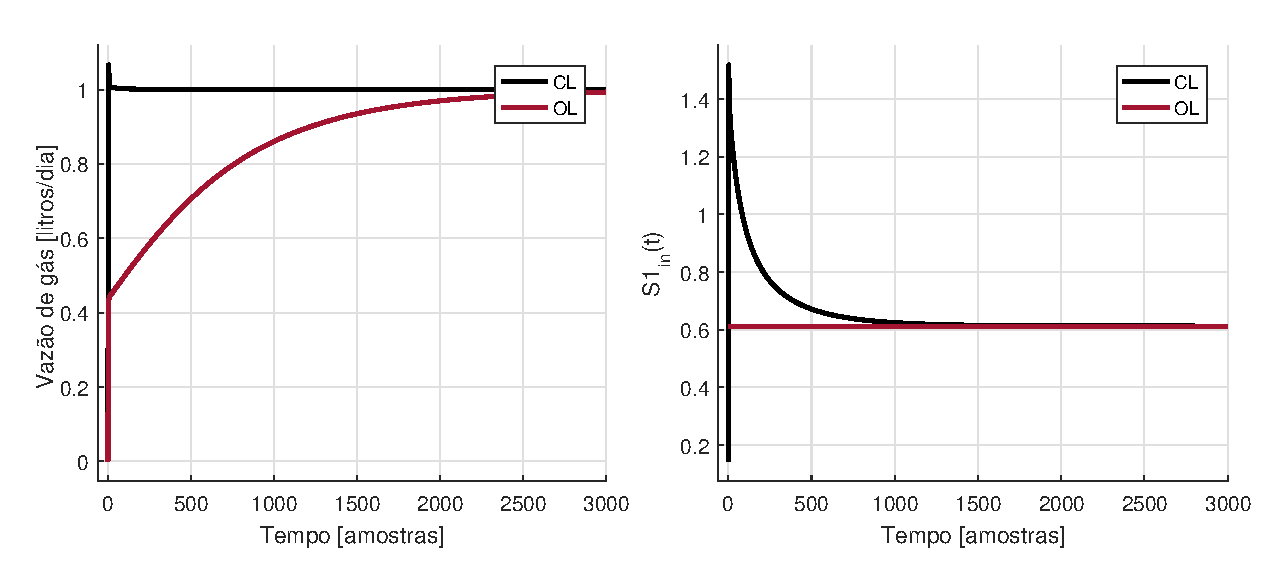
\includegraphics[width=.9\linewidth]{comparacao.eps}
\captionof{figure}{Comparação entre o desempenho em simulação do sistema em malha aberta (OL) em malha fechada (CL)} \label{sim}
\end{center}


%Fazendo pequenas alterações no modelo do biorreator em malha aberta - incluindo a adição de uma equação corresponde à integral do erro de seguimento à referência - o sistema em malha fechada pode ser facilmente representado no espaço de estados. A estabilidade do sistema em malha fechada, então, pode ser avaliada determinando-se o espectro da matriz Jacobiana (\textit{Lyapunov's indirect method}); o sistema será estável se, e somente se, a parte real de todos os autovalores é negativa. 

 
%Para o controle do processo, foi implementada a lei de controle apresentada na Equação %\ref{eq:lei_controle}. O sistema em malha fechada pode ser representado no espaço de estados através da adição de uma sexta equação e de alguns termos nas equações do modelo em  malha aberta apresentado adicionalmente.

%\begin{gather}
%y(t) = k_p \cdot (r(t)-q_m(t)) + k_i \cdot \int_{0}^{t} r(\tau)-q_m(\tau) d\tau  %%\label{eq:lei_controle}
%\end{gather} 
   
%\subsection*{Manipulação dos dados experimentais}
%Para a utilização dos dados do biorreator, foi necessário o desenvolvimento de um programa que processasse e manipulasse os dados de escrita do microcontrolador associado ao sensor de medição. Como a vazão do gás do reator é registrada de forma discreta pelos sensores óticos, procedeu-se o agrupamento dos dados em intervalos de amostragem $T$ e o seu registro em um arquivo que pudesse ser facilmente manipulado em Matlab.



%\begin{center}
%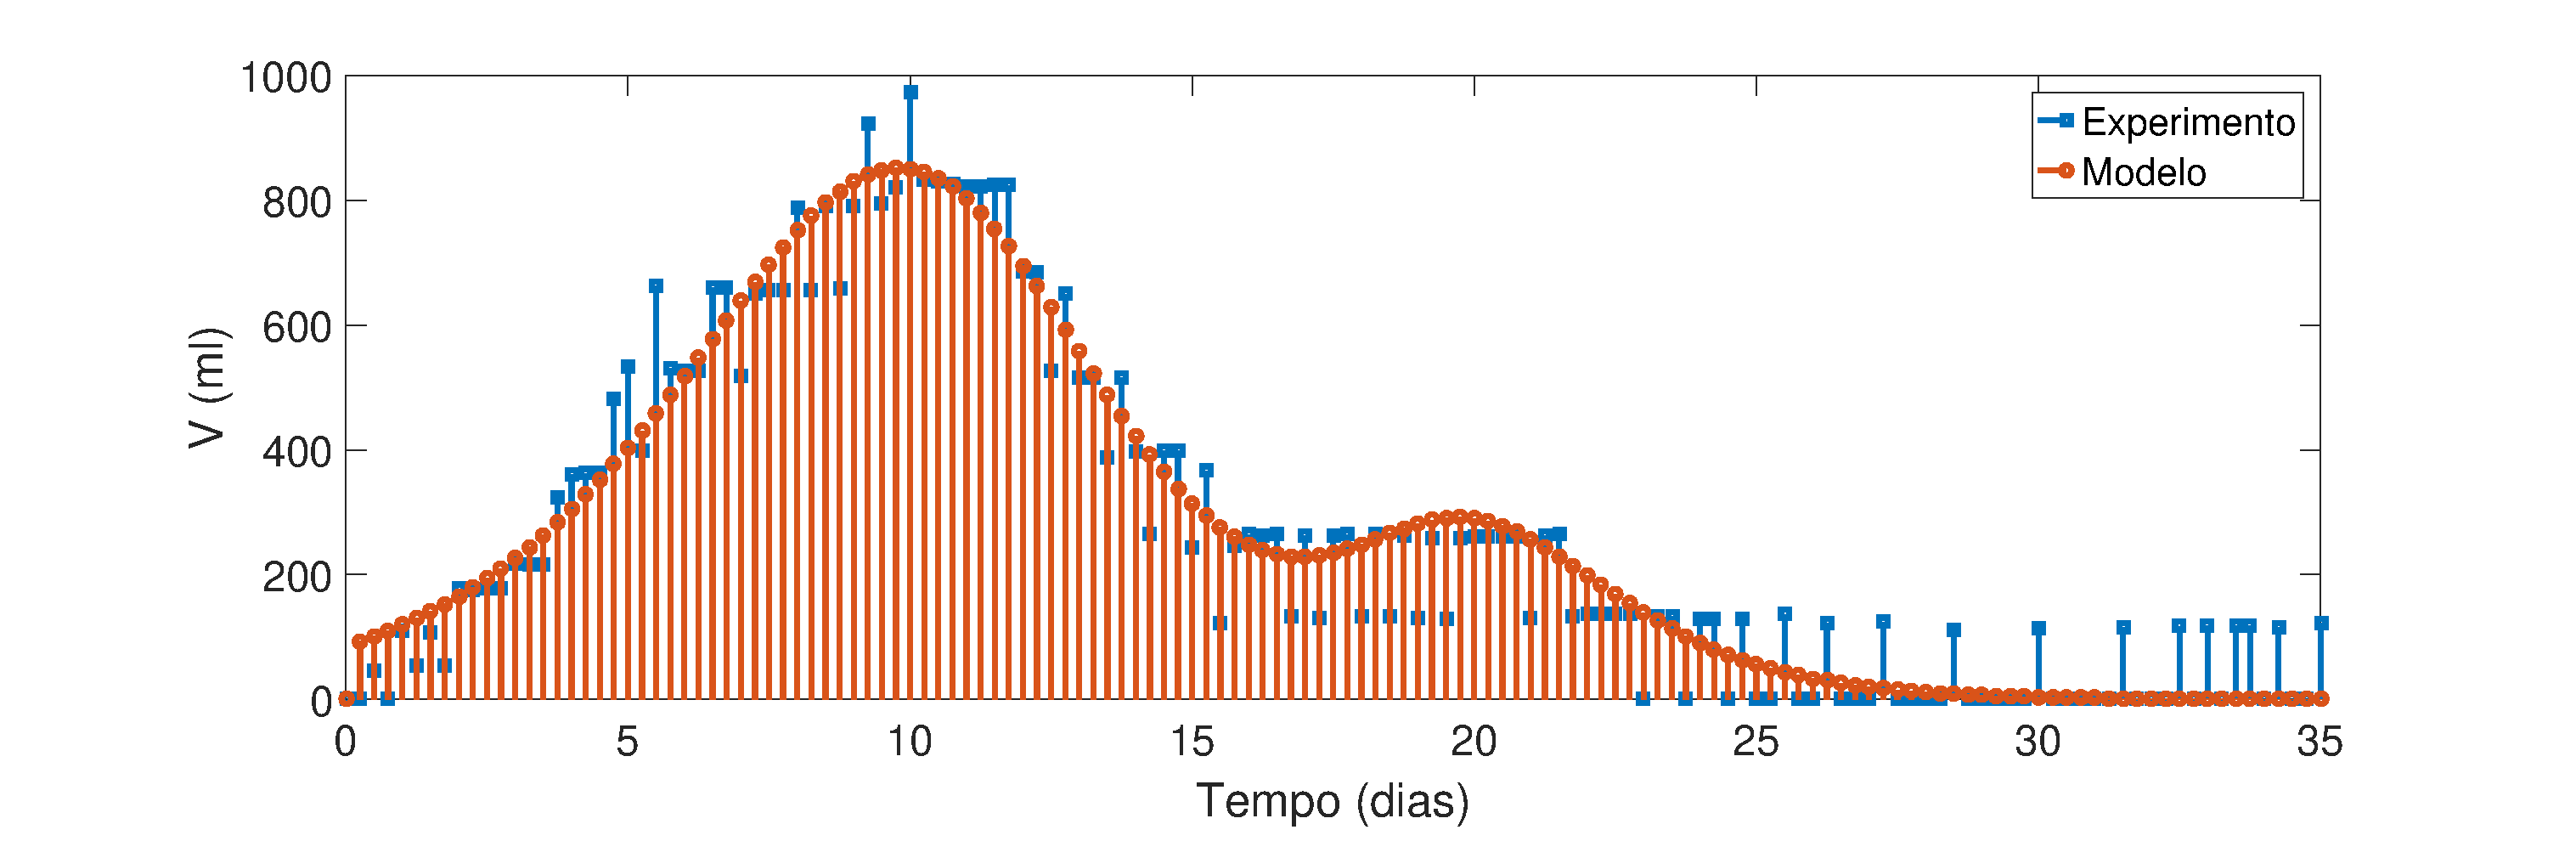
\includegraphics[width=0.8\linewidth]{simulacao2.eps}
%\captionof{figure}{ Comparação entre a simulação numérica do modelo do biorreator e os dados reais.}
%\end{center}

%----------------------------------------------------------------------------------------
%	CONCLUSIONS
%----------------------------------------------------------------------------------------

\section*{Conclusões}
	Os resultados demonstram que a implementação de um controlador PI (proporcional-integral) proporciona significativa melhoria de desempenho em relação ao sistema em malha aberta. Além disso, provê robustez a perturbações externas e a pequenas variações paramétricas. A fim de aperfeiçoar os resultados obtidos, será necessária a implementação efetiva do controlador \textit{in situ}.

\color{DarkSlateGray} % Set the color back to DarkSlateGray for the rest of the content

 %----------------------------------------------------------------------------------------
%	REFERENCES
%----------------------------------------------------------------------------------------

%\nocite{*} % Print all references regardless of whether they were cited in the poster or not
%\bibliographystyle{plain} % Plain referencing style
%\bibliographystyle{unsrt}
%{\footnotesize
%\bibliography{references}}

  
-----------------------------------------------------------------------

\end{multicols}
\end{document}